%%%%%%%%%%%%%%%%%%%%%%%%%%%%%%%%%%%%%%%%%%%%%%%%%
% Chapter: Tools
%%%%%%%%%%%%%%%%%%%%%%%%%%%%%%%%%%%%%%%%%%%%%%%%%
\chapter{Tools and Debuggers}
\label{chap:api_tools}

The term \textit{tool} widely refers to non-computational programs executed by the user or system administrator on a command line. Tools almost always interact with either the \ac{SMS}, user applications, or both to perform administrative and support functions. For example, a debugger tool might be used to remotely control the processes of a parallel application, monitoring their behavior on a step-by-step basis. Historically, such tools were custom-written for each specific host environment due to the customized and/or proprietary nature of the environment's interfaces.

The advent of \ac{PMIx} offers the possibility for creating portable tools capable of interacting with multiple \acp{RM} without modification. Possible use-cases include:

\begin{itemize}
\item querying the status of scheduling queues and estimated allocation time for various resource options
\item job submission and allocation requests
\item querying of job status for executing applications
\item launching and monitoring applications
\end{itemize}

Enabling these capabilities requires some extensions to the \ac{PMIx} Standard (both in terms of \acp{API} and attributes), and utilization of client-side \acp{API} for more tool-oriented purposes.

The APIs and attributes are captured elsewhere.

This chapter focuses instead on providing tool developers with an overview of the support provided by \ac{PMIx} and to guide \ac{RM} vendors regarding roles and responsibilities of the \ac{RM} to support tools.

%%%%%%%%%%%%%%%%%%%%%%%%%%%%%%%%%%%%%%%%%%%%%%
%%%%%%%%%%%%%%%%%%%%%%%%%%%%%%%%%%%%%%%%%%%%%%
\section{Connection Mechanisms}
\label{chap:api_tools:cnct}

The key to supporting such uses lies in providing a mechanism by which a tool can connect to a \ac{PMIx} server. Application processes are able to connect because their local \ac{RM} daemon provides them with the necessary contact information upon execution. A command-line tool, however, isn't spawned by an \ac{RM} daemon, and therefore lacks the information required for rendezvous with a \ac{PMIx} server.

\subsection{Rendezvousing with a local server}

In all other cases, the PMIx tool library will attempt to connect to according to the following precedence chain:

if PMIX_SERVER_URI or PMIX_TCP_URI is given, then connection will be attempted to the server at the specified URI. Note that it is an error for both of these attributes to be specified. PMIX_SERVER_URI is the preferred method as it is more generalized — PMIX_TCP_URI is provided for those cases where the user specifically wants to use a TCP transport for the connection and wants to error out if it isn’t available or cannot succeed. The PMIx library will return an error if connection fails — it will not proceed to check for other connection options as the user specified a particular one to use

if PMIX_SERVER_PIDINFO was provided, then the tool will search under the directory provided by the PMIX_SERVER_TMPDIR environmental variable for a rendezvous file created by the process corresponding to that PID. The PMIx library will return an error if the rendezvous file cannot be found, or the connection is refused by the server

if PMIX_CONNECT_TO_SYSTEM is given, then the tool will search for a system-level rendezvous file created by a PMIx server in the directory specified by the PMIX_SYSTEM_TMPDIR environmental variable. If found, then the tool will attempt to connect to it. An error is returned if the rendezvous file cannot be found or the connection is refused.

if PMIX_CONNECT_SYSTEM_FIRST is given, then the tool will search for a system-level rendezvous file created by a PMIx server in the directory specified by the PMIX_SYSTEM_TMPDIR environmental variable. If found, then the tool will attempt to connect to it. In this case, no error will be returned if the rendezvous file is not found or connection is refused — the PMIx library will silently continue to the next option

by default, the tool will search the directory tree under the directory provided by the PMIX_SERVER_TMPDIR environmental variable for rendezvous files of PMIx servers, attempting to connect to each it finds until one accepts the connection. If no rendezvous files are found, or all contacted servers refuse connection, then the PMIx library will return an error.

Note that there can be multiple local servers - one from the system plus others from launchers. Review the precedence ordering and how the attributes can modify it.


\subsection{Connecting to a remote server}

Only mechanism is to provide the specific URI to connect to - perhaps add ability to specify node and execute the rendezvous protocol? Implementations must support connection to any daemon, if attribute specifies.


\subsection{Attaching to running jobs}

Connect to any daemon within the application's scope, or to a system-level daemon with access to that scope. Can discover that information by connecting first to a system-level daemon and querying about active applications, then connect to appropriate point. Once attached to the appropriate PMIx server, can interact with the application using any PMIx mechanism. Includes querying application and process status, query application internal counters and state that has been exposed via PMIx events, etc.


%%%%%%%%%%%%%%%%%%%%%%%%%%%%%%%%%%%%%%%%%%%%%%
%%%%%%%%%%%%%%%%%%%%%%%%%%%%%%%%%%%%%%%%%%%%%%
\section{Application Launch}
\label{chap:api_tools:launch}

Tool-directed launches can take two modes:

\begin{itemize}
    \item \emph{Direct launch} where the resource manager (RM) itself is directly responsible for launching all processes, including debugger daemons – i.e., there is no intermediate launcher such as mpiexec; and
    \item \emph{Indirect launch} where all processes are started via an intermediate launcher such as mpiexec and the resource manager (RM) itself is not involved in launching application processes or debugger daemons
\end{itemize}


\subsection{Direct launch}

In the direct-launch use-case, . The user invokes a tool (typically on a non-compute, or “head”, node) to launch their application. An allocation of resources may or may not have been made in advance – if not, then the spawn request must include allocation request information. Once invoked, the tool connects to a system-level PMIx server, typically hosted by the resource manager (RM), constructs a PMIx_Spawn command, and communicates that command to the server.

The system-level PMIx server “uplifts” the spawn request to its host RM daemon for processing. If an allocation must be made, then the host RM daemon is responsible for communicating that request to its associated scheduler. Once resources are available, the host RM initiates the launch process, sending the application launch command to its daemons on the allocated nodes. The remote daemons then start their local client processes and the debugger daemons, providing the latter with all information required for them to attach to their targets.

The RM must parse the spawn request for relevant directives, returning an error if any required directive cannot be supported. Whether the parsing occurs on the initial daemon, or on the remote compute-node daemons, is left to the RM.

In the following example, the debugger tool initially queries the host RM regarding two key areas of support:

    ability to co-launch debugger daemons with application processes – i.e., does the RM support combining debugger daemons with application descriptions in the same call to PMIx_Spawn? If not, then the debugger tool must issue two spawn requests, one for the application and the other for the debugger daemons
    debugger attach modes – i.e., does the RM support stopping the application at first instruction until the debugger daemon releases it? If not, then the debugger must either be instructed that the application will be stopping in its own internal location, or instruct the PMIx client library in the application to instead stop in PMIx_Init until the debugger daemon releases it

The example assumes that co-launch is not supported on this RM, and so it proceeds to construct two spawn commands, issuing the one to launch the debugger daemons once it has determined that the application has been successfully spawned. The example code then waits until it has been notified by the RM (via registration of an appropriate PMIx event handler) that the debugger and application have both completed.


\subsection{Indirect launch}


Controlling the launcher with "wait for directives"

In the indirect-launch use-case, the resource manager (RM) itself is not involved in launching application processes or debugger daemons. Indeed, in some cases the RM has no actual visibility of those processes, nor knowledge of their existence. Instead, processes are started via an intermediate launcher such as mpiexec (which we will use for this example). In turn, the intermediate launcher starts its own network of daemons (e.g., mpid) that assume responsibility for launching and supporting the job. The intermediate launcher may use the RM to launch the daemons, or ssh, depending on the precise implementation, environment, and user preferences.

A primary objective during the design of this operational mode is to avoid any requirement that the debugger parse and/or understand the command line of mpiexec. Thus, the focus is on cleanly passing all non-debugger options from the initial command line to mpiexec, using the PMIx tool-to-server connection to communicate any other directives.

In this operational mode, the user invokes a tool (typically on a non-compute, or “head”, node) that in turn uses mpiexec to launch their application – a typical command line might look like the following:


\$ dbgr -dbgoption mpiexec -n 32 ./myapp

The tool may subsequently invoke mpiexec by simply executing it from a command line (e.g., using the Posix “system” function), or it may fork/exec it, or may request that it be started by the RM using the PMIx_Spawn API. The above illustration uses the last method. Regardless of how it is started, the debugger sets the PMIX_LAUNCHER_PAUSE_FOR_TOOL in the environment of mpiexec or in the pmix_info_t array in the spawn command. This instructs mpiexec to pause after initialization so it can receive further instructions from the debugger. This might include a request to co-spawn debugger daemons along with the application, or further directives relating to the startup of the application (e.g., to LD_PRELOAD a library, or replace the launcher’s local spawn agent with one provided by the debugger).

As mpiexec starts up, it calls PMIx_server_init to setup its PMIx server. The server initialization includes writing a server-level rendezvous file that allows other processes (such as the originating debugger) to connect to the server. It then pauses, awaiting further instructions from the debugger.

Armed with the pid (returned by fork/exec or the “system” command) or the namespace (returned by PMIx_Spawn) of the executing mpiexec, the debugger tool utilizes the PMIx_tool_switch_server API to complete the connection to the mpiexec server. Note that:

    PMIx does not allow servers to initiate connections – thus, the debugger tool must initiate the connection to the mpiexec server.
    tools can only be connected to one server at a time. Therefore, if connected to the system-level server to use PMIx_Spawn to launch mpiexec, the debugger tool will be disconnected from that server and connected to the PMIx server in mpiexec

At this point, the debugger can execute any PMIx operation, including:

    query mpiexec capabilities;
    pass directives to configure application behavior – e.g., specifying the desired pause point where application processes shall wait for debugger release;
    request launch of debugger daemons, providing the appropriate pmix_app_t description
    specify a replacement fork/exec agent; and
    define/modify standard environmental variables for the application

Once ready to launch, mpiexec parses its command line to obtain a description of the desired job. An allocation of resources may or may not have been made in advance (either by the user, or by the tool prior to starting mpiexec)- if not, then mpiexec may itself utilize the PMIx_Alloc API to obtain one from the system-level PMIx server. Once resources are available, mpiexec initiates the launch process by first spawning its daemon network across the allocation – in the above diagram, this is done via ssh commands. After the daemons have launched and wired up, mpiexec sends an application launch command to its daemons, which then start their local client processes and debugger daemons, providing the latter with all information required for them to attach to their targets.

The following example illustrates how a debugger tool would execute an indirect launch using the mpiexec launcher from some supporting MPI library. There are a few points worth noting:

    the debugger tool itself doesn’t need to know if mpiexec can co-launch the debugger daemons, or must launch the application and debugger daemons as separate operations. We require that mpiexec notify the tool when the entire spawn is completed
    the mpiexec launcher is required to provide each debugger daemon with the nspace of the target application it is to debug. This is done via a job-level PMIx attribute that the debugger daemon can query upon startup. Once the daemon has the target nspace, it can obtain the local (and complete, if desired) table of process pid’s and hostnames (commonly called the proctable) by querying it from the local PMIx server hosted in the local mpid
    the debugger tool command-line parser does not need to identify the application to be executed. It can parse only its own options, taking everything else as being an opaque array of argv to be passed along
    the job-level information provided by mpiexec to the debugger daemons must include the mechanism by which the daemon can release the target application processes. This could include release via PMIx event notification (the precise notification code must be given), use of a specific signal, or some other mechanism. The debugger is free to terminate the job if it cannot support the given mechanism


%%%%%%%%%%%%%%%%%%%%%%%%%%%%%%%%%%%%%%%%%%%%%%
%%%%%%%%%%%%%%%%%%%%%%%%%%%%%%%%%%%%%%%%%%%%%%
\section{IO Forwarding}
\label{chap:api_tools:iof}


Underlying the operation of many tools is a common need to forward stdin from the tool to targeted processes, and to return stdout/stderr from those processes to the tool (e.g., for display on the user’s console). Historically, each tool developer was responsible for creating their own \ac{IO} forwarding subsystem. However, the introduction of \ac{PMIx} as a standard mechanism for interacting between applications and the host environment has made it possible to relieve tool developers of this burden.

This section defines functions by which tools can request forwarding of input/output to/from other processes and serves as a design guide to:

\begin{itemize}
    \item provide tool developers with an overview of the expected behavior of the \ac{PMIx} \ac{IO} forwarding support;
    \item guide \ac{RM} vendors regarding roles and responsibilities expected of the \ac{RM} to support \ac{IO} forwarding; and
    \item provide insight into the thinking of the \ac{PMIx} community behind the definition of the \ac{PMIx} \ac{IO} forwarding \acp{API}
\end{itemize}

Note that the forwarding of \ac{IO} via \ac{PMIx} requires that both the host environment and the tool support \ac{PMIx}, but does not impose any similar requirements on the application itself.

\advicermstart
The responsibility of the host environment in forwarding of \ac{IO} falls into the following areas:

\begin{itemize}
    \item Capturing output from specified child processes
    \item Forwarding that output to the host of the \ac{PMIx} server library that requested it
    \item Delivering that payload to the \ac{PMIx} server library via the \refapi{PMIx_server_IOF_deliver} \ac{API} for final dispatch
\end{itemize}

\advicermend

\adviceimplstart
It is the responsibility of the \ac{PMIx} library to buffer, format, and deliver the payload to the requesting client. This

requires caching of output until forwarding registration received. Add attribute for setting cache side - it will be total number of messages to hold, intended to allow more flexible memory management. Not per source, but total across all jobs within the scope of that set of RM daemons - probably need to clarify the scope. Oldest message shall be dropped to make room for latest message, if required.

\adviceimplend

%%%%%%%%%%%
\subsection{\code{Forwarding Stdout/Stderr}}

At an appropriate point in its operation (usually during startup), a tool will utilize the \refapi{PMIx_tool_init} function to connect to a \ac{PMIx} server. The \ac{PMIx} server can be hosted by an \ac{SMS} daemon or could be embedded in a library-provided starter program such as \textit{mpiexec} - in terms of \ac{IO} forwarding, the operations remain the same either way. For purposes of this discussion, we will assume the server is in an \ac{SMS} daemon and that the application processes are directly launched by the \ac{SMS} (see diagram at right).

\begin{wrapfigure}{r}{75mm}
  \begin{center}
    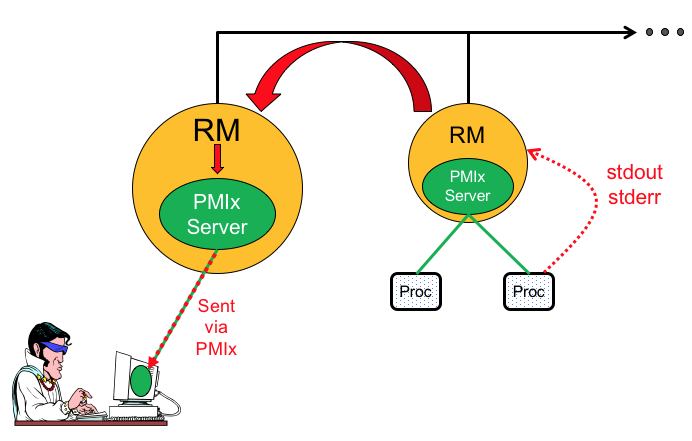
\includegraphics[clip,width=0.98\linewidth]{figs/output.png}
  \end{center}
    \caption{Forwarding stdout/stderr}
    \label{fig:stdouterr}
\end{wrapfigure}

Once the tool has connected to the target server, it can request that processes be spawned on its behalf and/or that output from a specified set of existing processes in a given executing application be forwarded to it. Requests to forward output from processes being spawned by the tool should be included in calls to the \refapi{PMIx_Spawn} \ac{API} using the \refattr{PMIX_FWD_STDOUT} and/or \refattr{PMIX_FWD_STDERR} attributes. This alleviates

Two modes are supported for the latter case of catching output from existing processes:

\begin{itemize}
    \item PMIX_IOF_COPY – deliver a copy of the output to the tool, letting the stream continue to also be delivered to the default location. This allows the tool to “tap” into the output stream without redirecting it from its current final destination
    \item PMIX_IOF_REDIRECT – intercept the output stream and deliver to the requesting tool instead of its current final destination. This might be used, for example, during a debugging procedure to avoid “polluting” the application’s results file. The original output stream destination is restored upon termination of the tool
\end{itemize}

Application processes are the children of the local SMS (typically, the local RM daemon) and not directly related to the PMIx server itself. Thus, it is the responsibility of the local SMS to collect the child’s output – usually done by capturing the relevant file descriptors at fork/exec of the child process – and the PMIx server on the remote nodes is not involved in this process. Once captured, the host SMS is responsible for returning the output to the SMS daemon serving the tool. This typically will be the daemon co-located with the tool, but this isn’t required.

Once the output reaches the serving SMS daemon, the daemon passes the output to its embedded PMIx server via the PMIx_IOF_push function whose parameter list includes the identifier of the source process and the IOF channel of the provided data. The PMIx server will transfer the data to the tool’s client library, which will in turn output it to the screen.

When registering to receive output, the tool can specify several formatting options to be used on the resulting output stream. These include:

    PMIX_IOF_TAG – output is prefixed with the nspace,rank of the source and a string identifying the channel (stdout, stderr, etc.)
    PMIX_IOF_TIMESTAMP – output is marked with the time at which the data was received by the tool (note that this will differ from the time at which it was actually output by the source)
    PMIX_IOF_XML_OUTPUT – output is to be formatted in XML

The PMIx client in the tool will format the output stream. Note that output from multiple processes will often be interleaved due to variations in arrival time - ordering of output is \emph{not} guaranteed across processes and/or nodes.

%%%%%%%%%%%
\subsubsection{\code{PMIx_IOF_pull}}
\declareapi{PMIx_IOF_pull}

%%%%
\summary

Register to receive output forwarded from a set of remote processes.

%%%%
\format

\versionMarker{3.0}
\cspecificstart
\begin{codepar}
pmix_status_t
PMIx_IOF_pull(const pmix_proc_t procs[], size_t nprocs,
              const pmix_info_t directives[], size_t ndirs,
              pmix_iof_channel_t channel, pmix_iof_cbfunc_t cbfunc,
              pmix_hdlr_reg_cbfunc_t regcbfunc, void *regcbdata)
\end{codepar}
\cspecificend

\begin{arglist}
\argin{procs}{Array of proc structures identifying desired source processes (array of handles)}
\argin{nprocs}{Number of elements in the \refarg{procs} array (integer)}
\argin{directives}{Array of \refstruct{pmix_info_t} structures (array of handles)}
\argin{ndirs}{Number of elements in the \refarg{directives} array (integer)}
\argin{channel}{Bitmask of IO channels included in the request (\refstruct{pmix_iof_channel_t})}
\argin{cbfunc}{Callback function for delivering relevant output (\refapi{pmix_iof_cbfunc_t} function reference)}
\argin{regcbfunc}{Function to be called when registration is completed (\refapi{pmix_hdlr_reg_cbfunc_t} function reference)}
\argin{regcbdata}{Data to be passed to the \refarg{regcbfunc} callback function (memory reference)}
\end{arglist}

Returns \refconst{PMIX_SUCCESS} or a negative value corresponding to a PMIx error constant. In the event the function returns an error, the \refarg{regcbfunc} will \textit{not} be called.

\reqattrstart
The following attributes are required for \ac{PMIx} libraries that support \ac{IO} forwarding:

\pastePRIAttributeItem{PMIX_IOF_CACHE_SIZE}
\pastePRIAttributeItem{PMIX_IOF_DROP_OLDEST}
\pastePRIAttributeItem{PMIX_IOF_DROP_NEWEST}

\reqattrend

\optattrstart
The following attributes are optional for \ac{PMIx} libraries that support \ac{IO} forwarding:

\pastePRIAttributeItem{PMIX_IOF_BUFFERING_SIZE}
\pastePRIAttributeItem{PMIX_IOF_BUFFERING_TIME}
\pastePRIAttributeItem{PMIX_IOF_TAG_OUTPUT}
\pastePRIAttributeItem{PMIX_IOF_TIMESTAMP_OUTPUT}
\pastePRIAttributeItem{PMIX_IOF_XML_OUTPUT}

\optattrend

%%%%
\descr

Register to receive output forwarded from a set of remote processes.

\adviceuserstart
Providing a \code{NULL} function pointer for the \refarg{cbfunc} parameter will cause output for the indicated channels to be written to their corresponding stdout/stderr file descriptors. Use of \refconst{PMIX_RANK_WILDCARD} to specify all processes in a given namespace is supported but should be used carefully due to bandwidth considerations.
\adviceuserend

%%%%%%%%%%%
\subsubsection{\code{PMIx_IOF_deregister}}
\declareapi{PMIx_IOF_deregister}

%%%%
\summary

Deregister from output forwarded from a set of remote processes.

%%%%
\format

\versionMarker{3.0}
\cspecificstart
\begin{codepar}
pmix_status_t
PMIx_IOF_deregister(size_t iofhdlr,
                    const pmix_info_t directives[], size_t ndirs,
                    pmix_op_cbfunc_t cbfunc, void *cbdata)
\end{codepar}
\cspecificend

\begin{arglist}
\argin{iofhdlr}{Registration number returned from the \refapi{pmix_hdlr_reg_cbfunc_t} callback from the call to \refapi{PMIx_IOF_pull} (\code{size_t})}
\argin{directives}{Array of \refstruct{pmix_info_t} structures (array of handles)}
\argin{ndirs}{Number of elements in the \refarg{directives} array (integer)}
\argin{cbfunc}{Callback function to be called when deregistration has been completed. (function reference)}
\argin{cbdata}{Data to be passed to the \refarg{cbfunc} callback function (memory reference)}
\end{arglist}

Returns one of the following:

\begin{itemize}
    \item \refconst{PMIX_SUCCESS}, indicating that the request is being processed by the host environment - result will be returned in the provided \refarg{cbfunc}. Note that the library \emph{must not} invoke the callback function prior to returning from the \ac{API}.
    \item \refconst{PMIX_OPERATION_SUCCEEDED}, indicating that the request was immediately processed and returned \textit{success} - the \refarg{cbfunc} will \textit{not} be called
    \item a PMIx error constant indicating either an error in the input or that the request was immediately processed and failed - the \refarg{cbfunc} will \textit{not} be called
\end{itemize}

%%%%
\descr

Deregister from output forwarded from a set of remote processes.

\adviceimplstart
Any currently buffered \ac{IO} should be flushed upon receipt of a deregistration request. All received \ac{IO} after receipt of the request shall be discarded.
\adviceimplend


%%%%%%%%%%%
\subsection{\code{Forwarding stdin}}

A tool is not necessarily a child of the \ac{RM} as it may have been started directly from the command line. Thus, provision must be made for the tool to collect its stdin and pass it to the host \ac{RM} (via the \ac{PMIx} server) for forwarding. Two methods of support for forwarding of stdin are defined:

\begin{wrapfigure}{r}{75mm}
  \begin{center}
    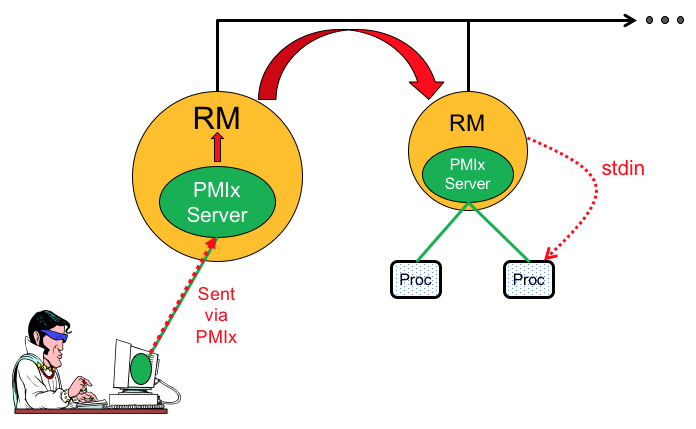
\includegraphics[clip,width=0.98\linewidth]{figs/input.png}
  \end{center}
    \caption{Forwarding stdin}
    \label{fig:stdin}
\end{wrapfigure}

\begin{itemize}
    \item internal collection by the \ac{PMIx} tool library itself. This is requested via the \refattr{PMIX_IOF_PUSH_STDIN} attribute in the \refapi{PMIx_IOF_push} call. When this mode is selected, the tool library begins collecting all stdin data and internally passing it to the local server for distribution to the specified target processes. All collected data is sent to the same targets until stdin is closed, or a subsequent call to \refapi{PMIx_IOF_push} is made that includes the \refattr{PMIX_IOF_COMPLETE} attribute indicating that forwarding of stdin is to be terminated.
    \item external collection directly by the tool. It is assumed that the tool will provide its own code/mechanism for collecting its stdin as the tool developers may choose to insert some filtering and/or editing of the stream prior to forwarding it. In addition, the tool can directly control the targets for the data on a per-call basis – i.e., each call to \refapi{PMIx_IOF_push} can specify its own set of target recipients for that particular ``blob'' of data. Thus, this method provides maximum flexibility, but requires that the tool developer provide their own code to capture stdin.
\end{itemize}

Note that it is the responsibility of the resource manager to forward data to the host where the target process(es) are executing, and for the host daemon on that node to deliver the data to the stdin of target process(es) via the typical pipe. The \ac{PMIx} server on the remote node is \emph{not} involved in this process. Systems that do not support forwarding of stdin shall return \refconst{PMIX_ERR_NOT_SUPPORTED} in response to a forwarding request.

\adviceimplstart
It is recognized that scalable forwarding of stdin represents a significant challenge. A high quality implementation will at least handle a ``send-to-1'' model whereby stdin is forwarded to a single identified process, and an additional ``send-to-all'' model where stdin is forwarded to all processes in the application. Other models (e.g., forwarding stdin to an arbitrary subset of processes) are left to the discretion of the implementor.
\adviceimplend

\adviceuserstart
Stdin buffering by the \ac{RM} and/or \ac{PMIx} library can be problematic. If the targeted recipient is slow reading data (or decides never to read data), then the data must be buffered in some intermediate daemon or the local \ac{PMIx} server itself. Thus, piping a large amount of data into stdin can result in a very large memory footprint in the system management stack. This is further exacerbated when targeting multiple recipients as the buffering problem, and hence the resulting memory footprint, is compounded. Best practices, therefore, typically focus on reading of input files by application processes as opposed to forwarding of stdin.
\adviceuserend

%%%%%%%%%%%
\subsubsection{\code{PMIx_IOF_push}}
\declareapi{PMIx_IOF_push}

%%%%
\summary

Push data collected locally (typically from stdin or a file) to stdin of the target recipients.

%%%%
\format

\versionMarker{3.0}
\cspecificstart
\begin{codepar}
pmix_status_t
PMIx_IOF_push(const pmix_proc_t targets[], size_t ntargets,
              pmix_byte_object_t *bo,
              const pmix_info_t directives[], size_t ndirs,
              pmix_op_cbfunc_t cbfunc, void *cbdata)
\end{codepar}
\cspecificend

\begin{arglist}
\argin{targets}{Array of proc structures identifying desired target processes (array of handles)}
\argin{ntargets}{Number of elements in the \refarg{targets} array (integer)}
\argin{bo}{Pointer to \refstruct{pmix_byte_object_t} containing the payload to be delivered (handle)}
\argin{directives}{Array of \refstruct{pmix_info_t} structures (array of handles)}
\argin{ndirs}{Number of elements in the \refarg{directives} array (integer)}
\argin{directives}{Array of \refstruct{pmix_info_t} structures (array of handles)}
\argin{cbfunc}{Callback function to be called when operation has been completed. (\refapi{pmix_op_cbfunc_t} function reference)}
\argin{cbdata}{Data to be passed to the \refarg{cbfunc} callback function (memory reference)}
\end{arglist}

Returns one of the following:

\begin{itemize}
    \item \refconst{PMIX_SUCCESS}, indicating that the request is being processed by the host environment - result will be returned in the provided \refarg{cbfunc}. Note that the library \emph{must not} invoke the callback function prior to returning from the \ac{API}.
    \item \refconst{PMIX_OPERATION_SUCCEEDED}, indicating that the request was immediately processed and returned \textit{success} - the \refarg{cbfunc} will \textit{not} be called
    \item a PMIx error constant indicating either an error in the input or that the request was immediately processed and failed - the \refarg{cbfunc} will \textit{not} be called
\end{itemize}

\reqattrstart
The following attributes are required for \ac{PMIx} libraries that support \ac{IO} forwarding:

\pastePRIAttributeItem{PMIX_IOF_CACHE_SIZE}
\pastePRIAttributeItem{PMIX_IOF_DROP_OLDEST}
\pastePRIAttributeItem{PMIX_IOF_DROP_NEWEST}

\reqattrend

\optattrstart
The following attributes are optional for \ac{PMIx} libraries that support \ac{IO} forwarding:

\pastePRIAttributeItem{PMIX_IOF_BUFFERING_SIZE}
\pastePRIAttributeItem{PMIX_IOF_BUFFERING_TIME}

\optattrend

%%%%
\descr

Push data collected locally (typically from stdin or a file) to stdin of the target recipients.

\adviceuserstart
Execution of the \refarg{cbfunc} callback function serves as notice that the \ac{PMIx} library no longer requires the caller to maintain the \refarg{bo} data object - it does \textit{not} indicate delivery of the payload to the targets. Use of \refconst{PMIX_RANK_WILDCARD} to specify all processes in a given namespace is supported but should be used carefully due to bandwidth considerations.
\adviceuserend





\section{Querying Information}

Proctables et al.



%%%%%%%%%%%%%%%%%%%%%%%%%%%%%%%%%%%%%%%%%%%%%%%%%
